\documentclass[mathserif]{beamer}

\usepackage{subg}

%-----------------------------------------------------------------------
\usepackage{pdfpages}
\usepackage{array}
\usepackage{booktabs}
\usepackage[skins,breakable]{tcolorbox}
\usepackage{minibox}
\usepackage{mathtools}
\usepackage{amsmath}

% Avoid random transparencies in Adobe Acrobat
\usepackage{everypage}
\AddEverypageHook{%
  \makeatletter%
  \special{pdf: put @thispage <</Group << /S /Transparency /I true /CS /DeviceRGB>> >>}%
  \makeatother%
}%

\DeclareMathOperator*{\argmax}{arg\,max}

\newcommand{\todo}[1]{{\scriptsize\color{yellow}\textsc{[Todo]}}}

\newcommand{\qcite}[1]{{\scriptsize\color{col1}[#1]}}

\newcommand{\qbox}[1]{%
\begin{tcolorbox}[enhanced jigsaw,size=tight,hbox,boxsep=4pt,boxrule=1pt,coltext=black,colframe=col1light,colback=col1,opacityback=0.7,opacityframe=1]
\strut #1
\end{tcolorbox}%
}

\newcommand{\qboxa}[1]{%
\begin{tcolorbox}[enhanced jigsaw,size=tight,hbox,boxsep=4pt,boxrule=1pt,coltext=textcolor,colframe=col1,opacityback=0,opacityframe=1]
\strut #1
\end{tcolorbox}%
}

\newcommand{\qboxatight}[1]{%
\begin{tcolorbox}[enhanced jigsaw,size=fbox,hbox,boxsep=4pt,boxrule=1pt,coltext=textcolor,colframe=col1,opacityback=0,opacityframe=1,halign=center,valign=center,square,circular arc]
#1
\end{tcolorbox}%
}

\newcommand{\qboxb}[1]{%
\begin{tcolorbox}[enhanced jigsaw,size=tight,hbox,boxsep=4pt,boxrule=1pt,coltext=textcolor,colframe=col2,opacityback=0,opacityframe=1]
\strut #1
\end{tcolorbox}%
}

\newcommand{\qtheorem}[2]{%
\begin{tcolorbox}[enhanced jigsaw,size=tight,boxsep=7pt,boxrule=0.7pt,coltext=textcolor,colframe=col1,colback=col1,opacityback=0,opacityframe=1]
\begin{minipage}{\textwidth}
{\color{col1}\strut Theorem #1}\\[0.7em]
#2
\end{minipage}
\end{tcolorbox}%
}

\newcommand{\qlemma}[1]{%
\begin{tcolorbox}[enhanced jigsaw,size=tight,boxsep=7pt,boxrule=0.7pt,coltext=textcolor,colframe=col2,colback=col1,opacityback=0,opacityframe=1]
\begin{minipage}{\textwidth}
{\color{col2}\strut Lemma}\\[0.7em]
#1
\end{minipage}
\end{tcolorbox}%
}

\newcommand{\qsubtitle}[1]{%
{\color{col2}\textsc{#1}}
}

\newcommand{\qsource}[1]{%
{\color{col1}\tiny\hfill[#1]}
}

%-----------------------------------------------------------------------

\title[Discrete Sampling using Semigradient-based Product Mixtures]
{Discrete Sampling using Semigradient-based Product Mixtures}

\author[Alkis Gotovos]{}

\begin{document}

\setbeamertemplate{background canvas}{}
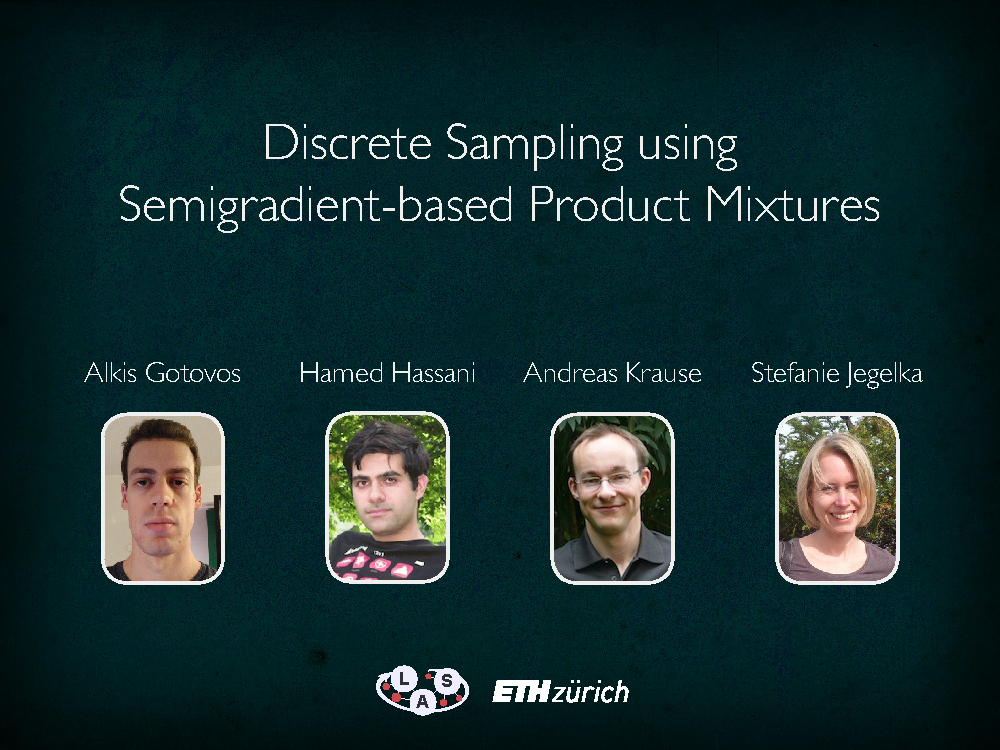
\includepdf[pages={1}]{title/title.pdf}
\setbeamertemplate{background canvas}{
\includegraphics[width=\paperwidth]{figures/bg_no_line.png}}

\begin{frame}{Modeling gene alterations}
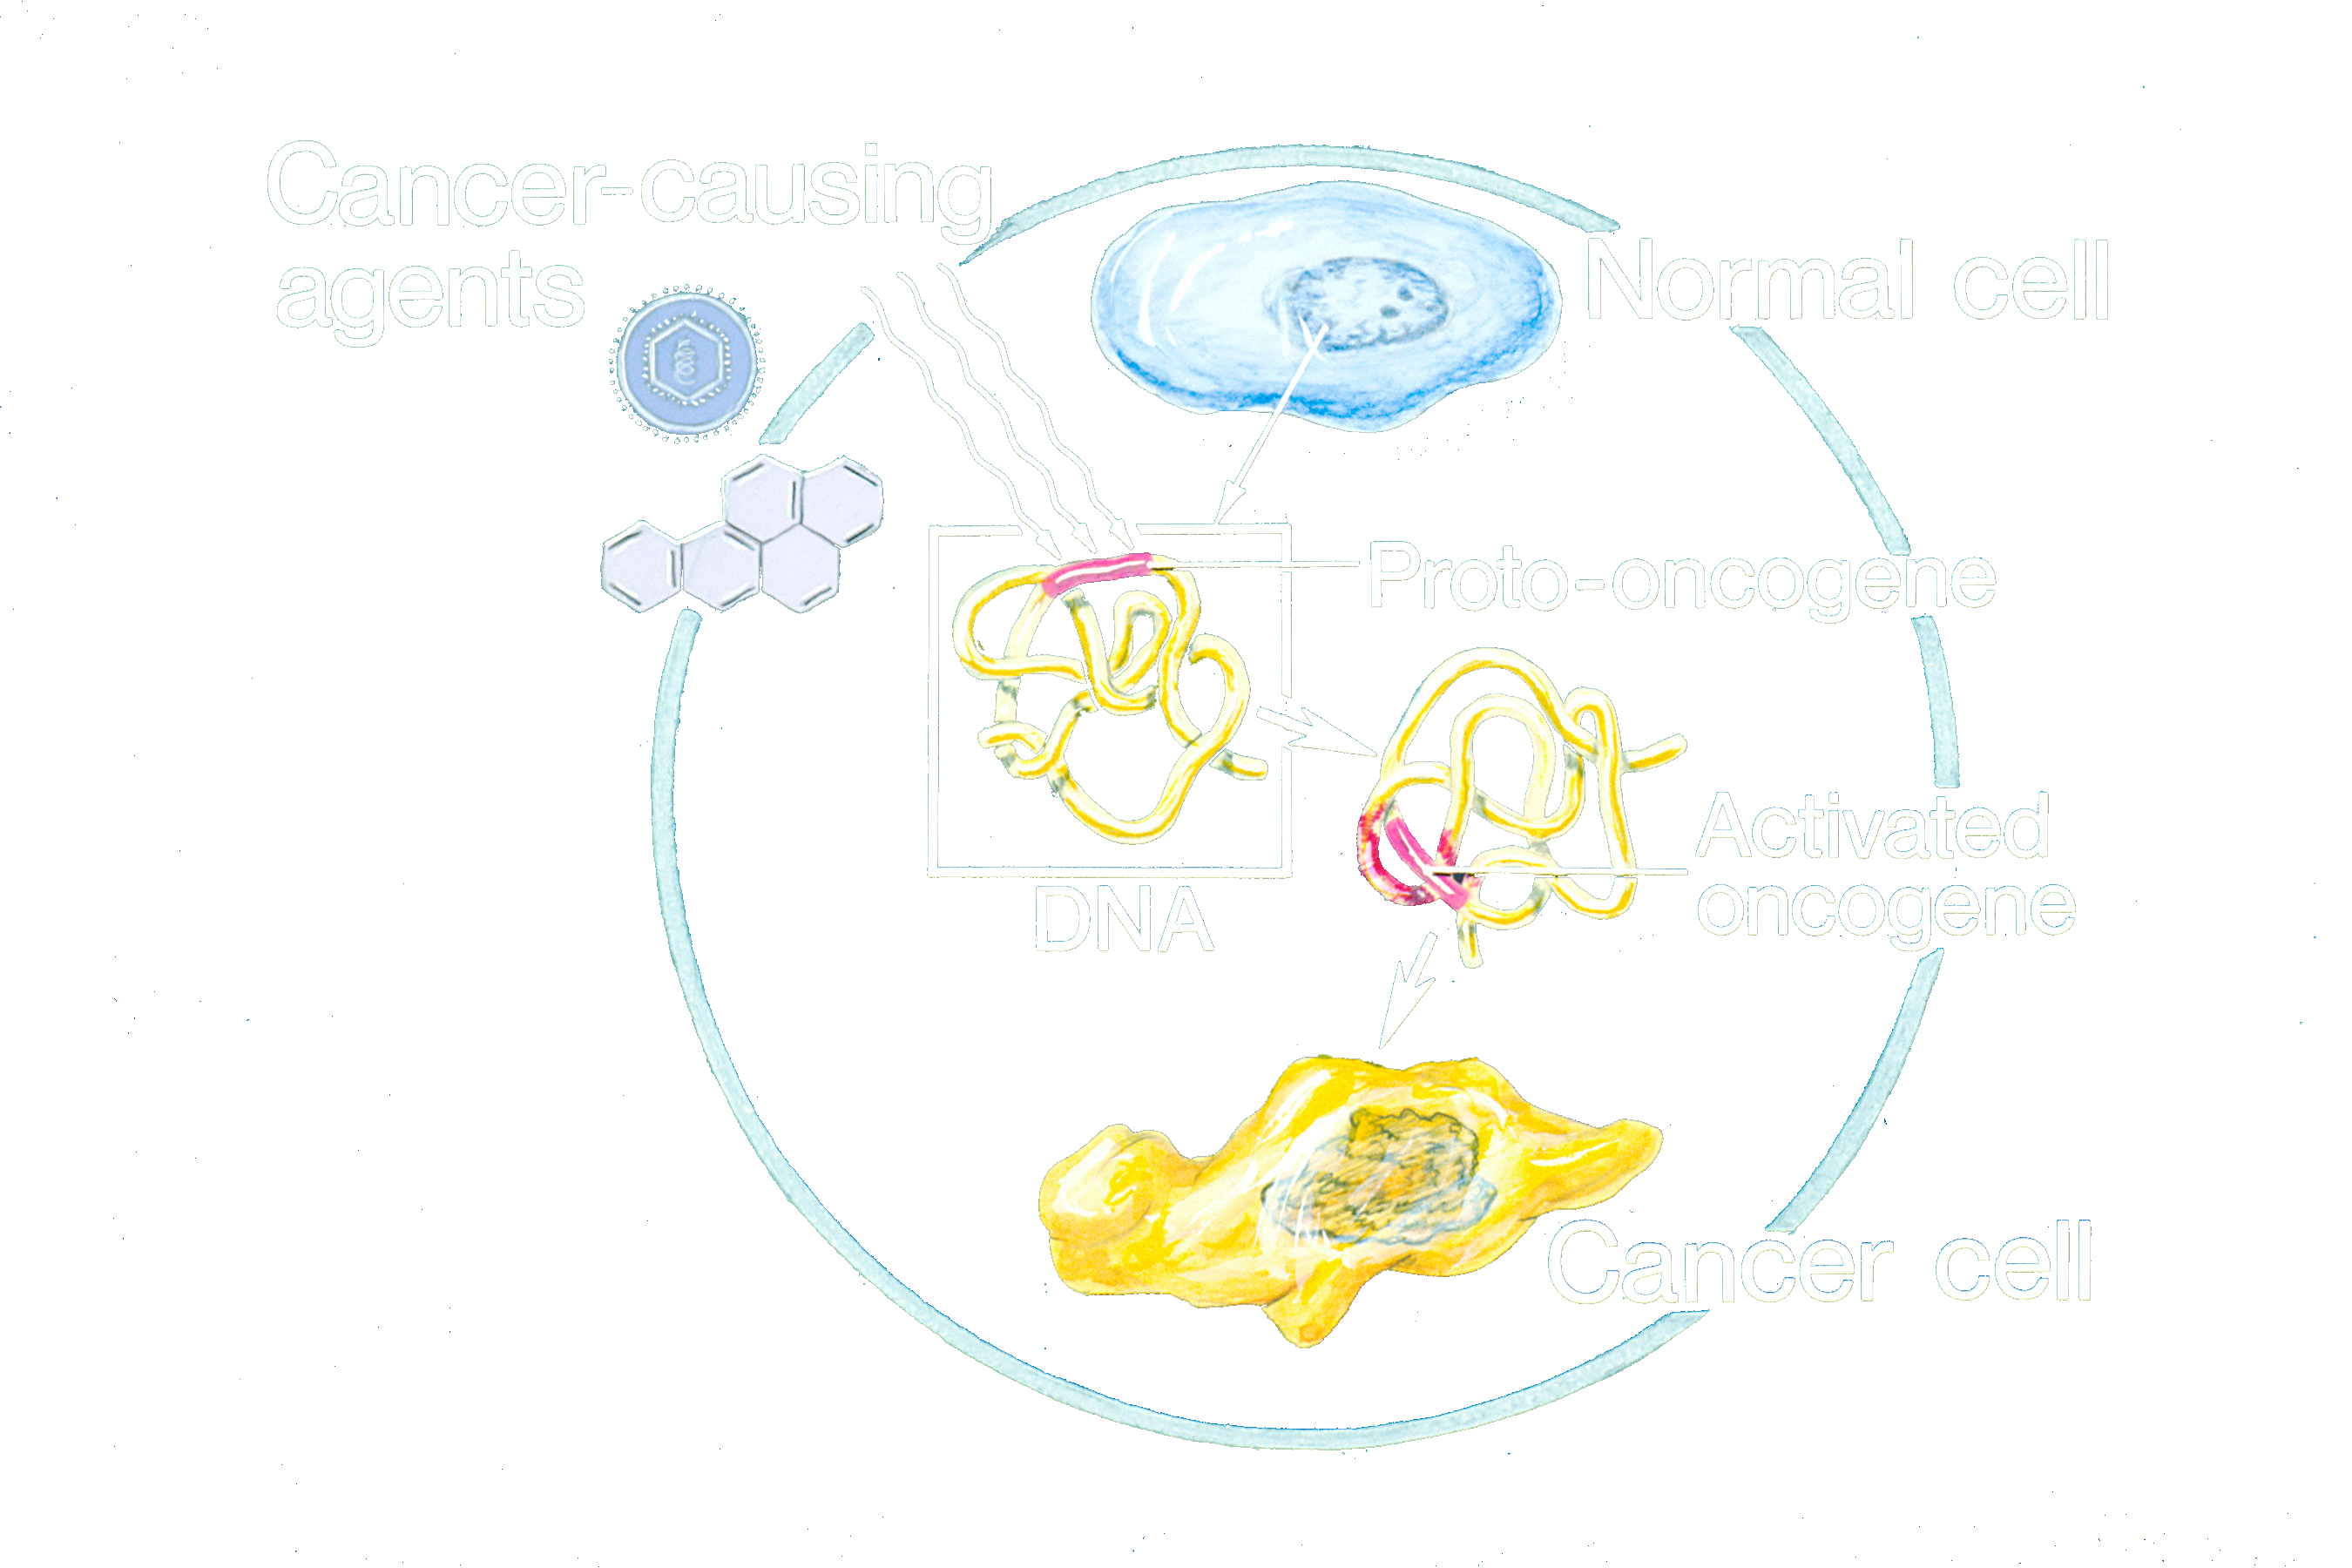
\includegraphics[width=3.7in]{figures/oncogene.png}\\
\qsource{\texttt{cancergenome.nih.gov}}
\end{frame}

\begin{frame}{Modeling gene alterations}
\centering
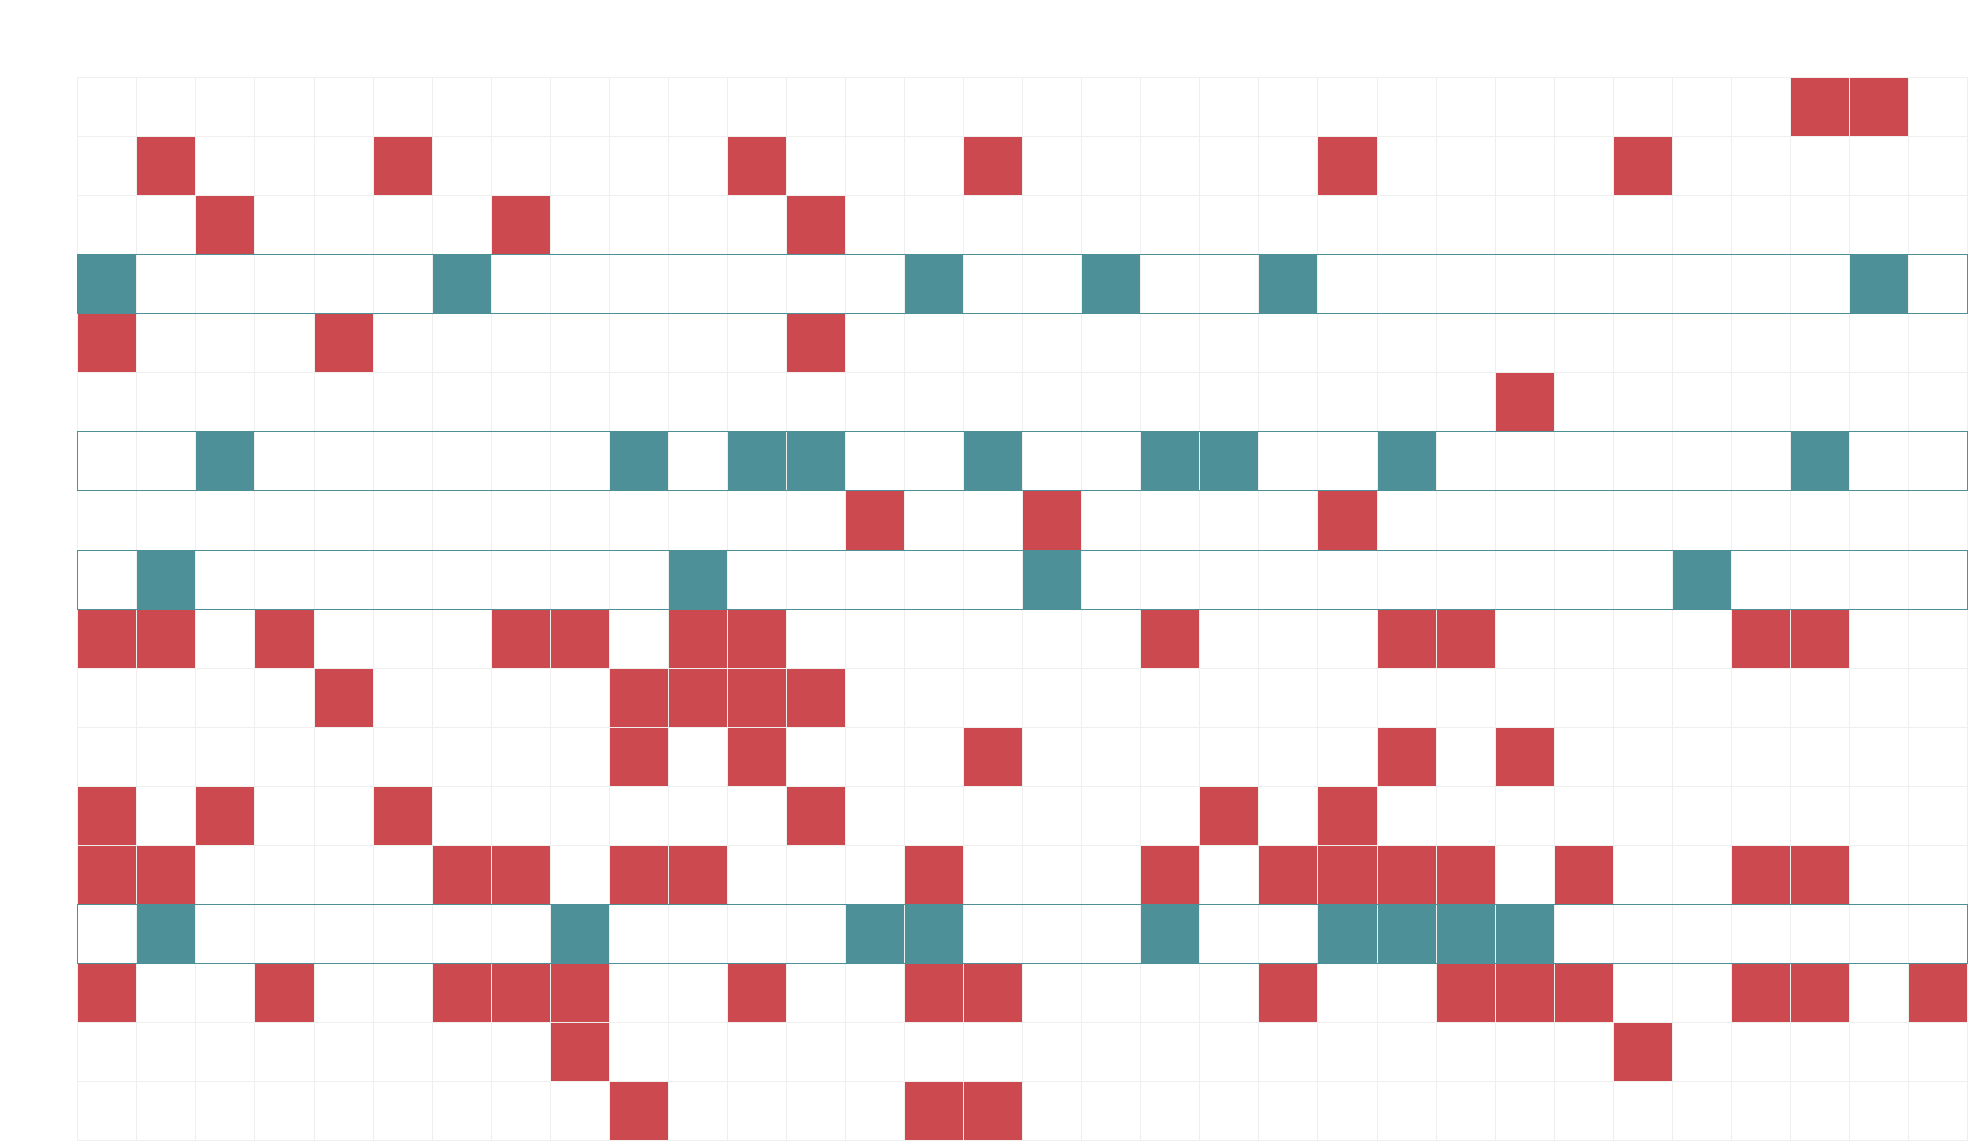
\includegraphics[width=\textwidth]{figures/grid_genes.pdf}
\end{frame}

\begin{frame}{Modeling gene alterations}
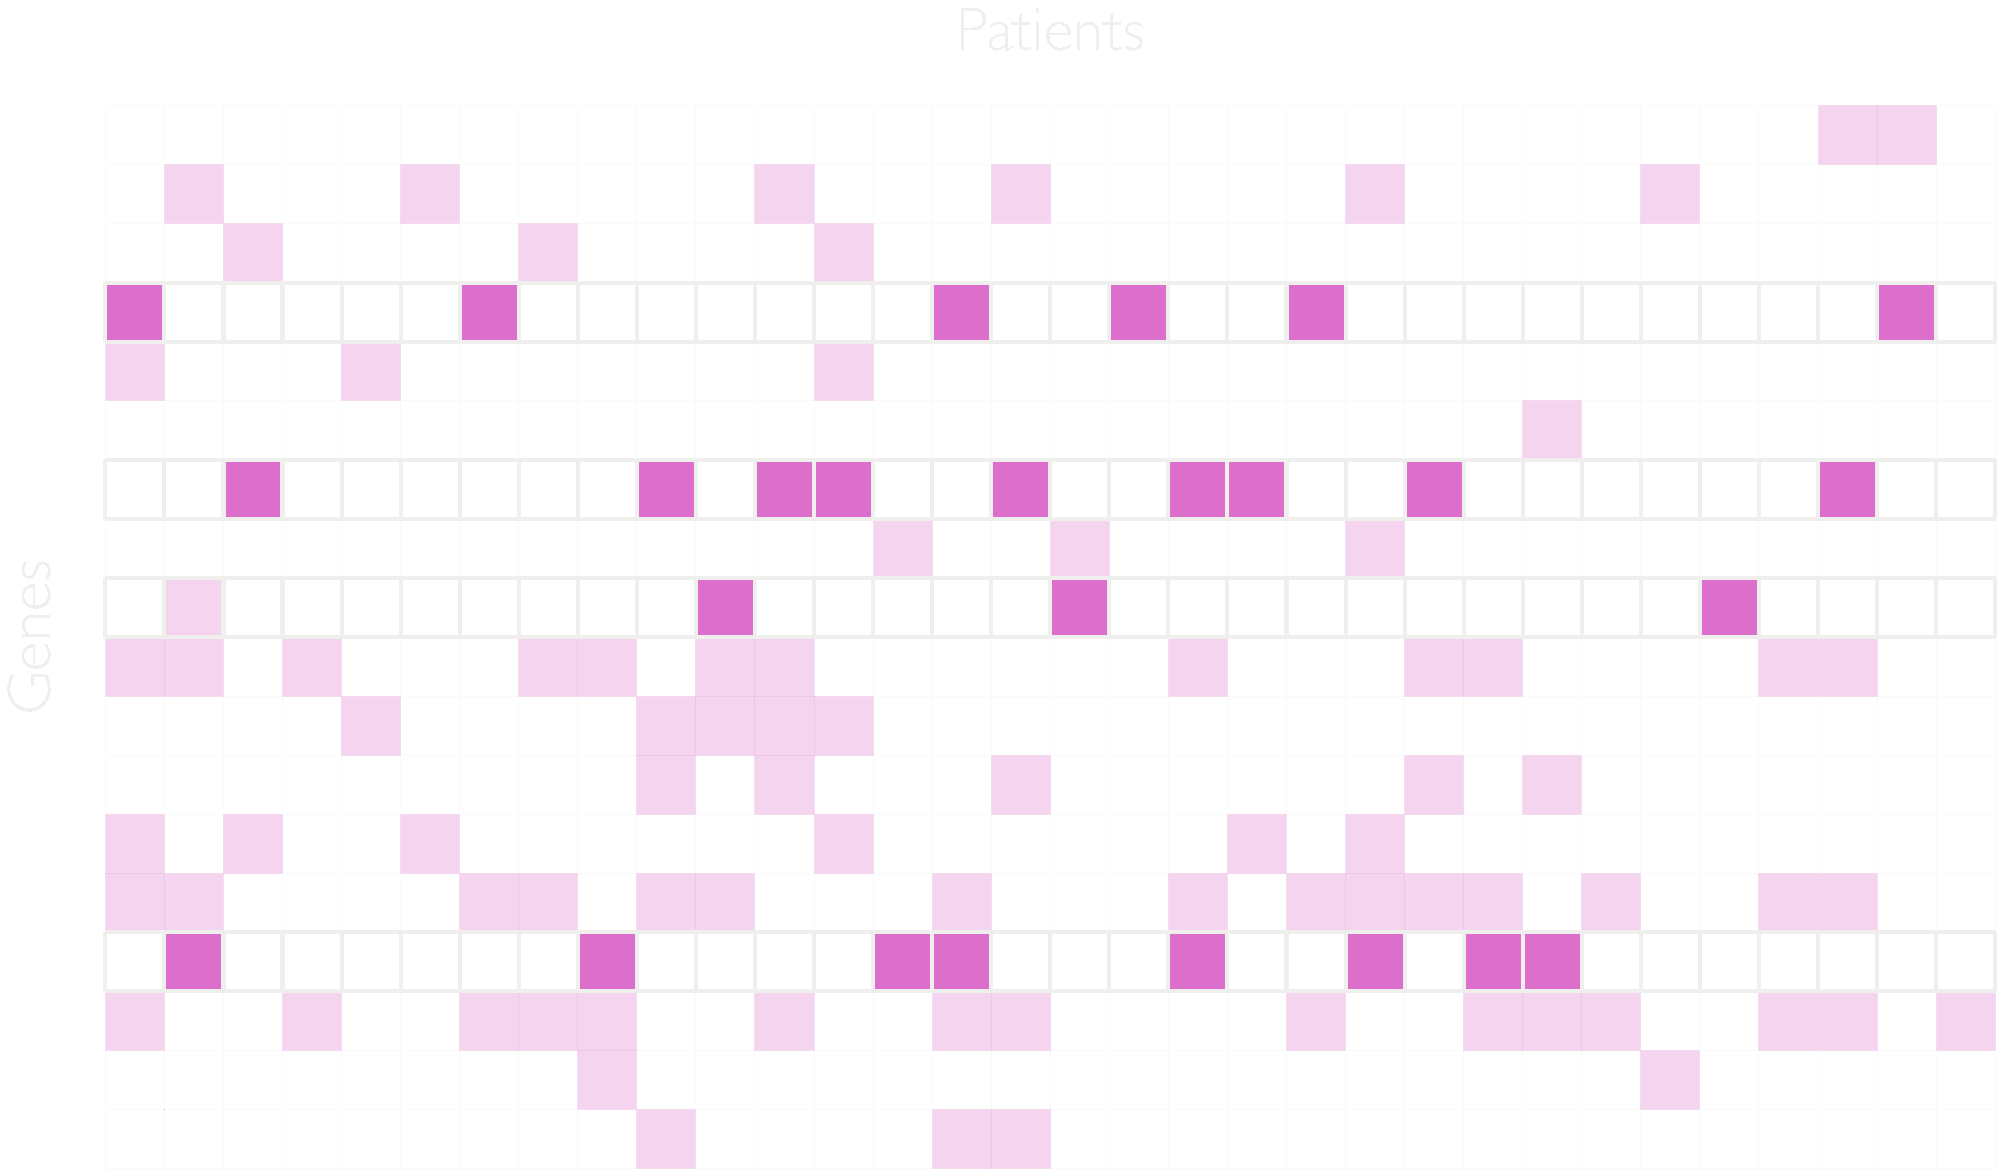
\includegraphics[width=\textwidth]{figures/grid_genes_muex.pdf}
\end{frame}

\begin{frame}{Modeling gene alterations}
\centering
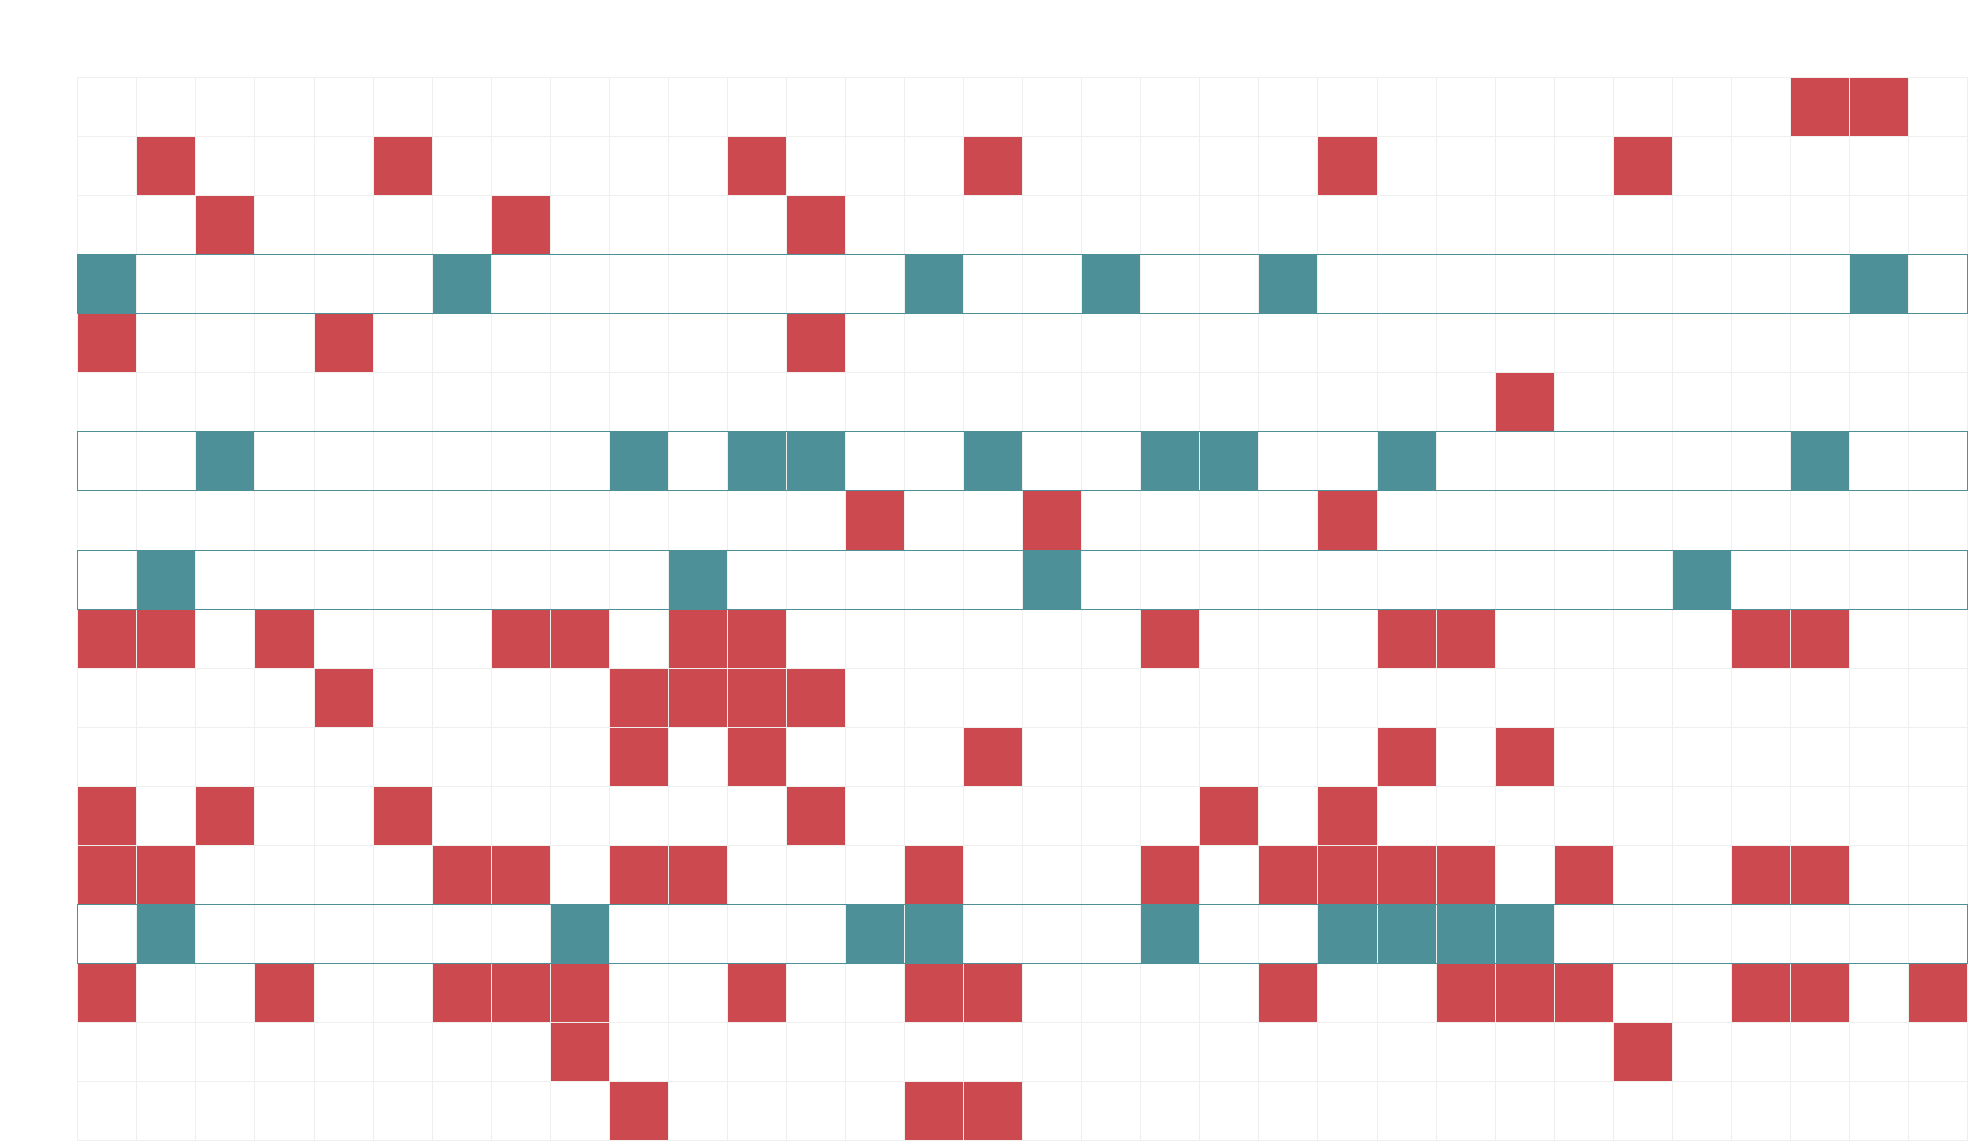
\includegraphics[width=\textwidth]{figures/grid_genes.pdf}
\end{frame}

\begin{frame}{Modeling gene alterations}
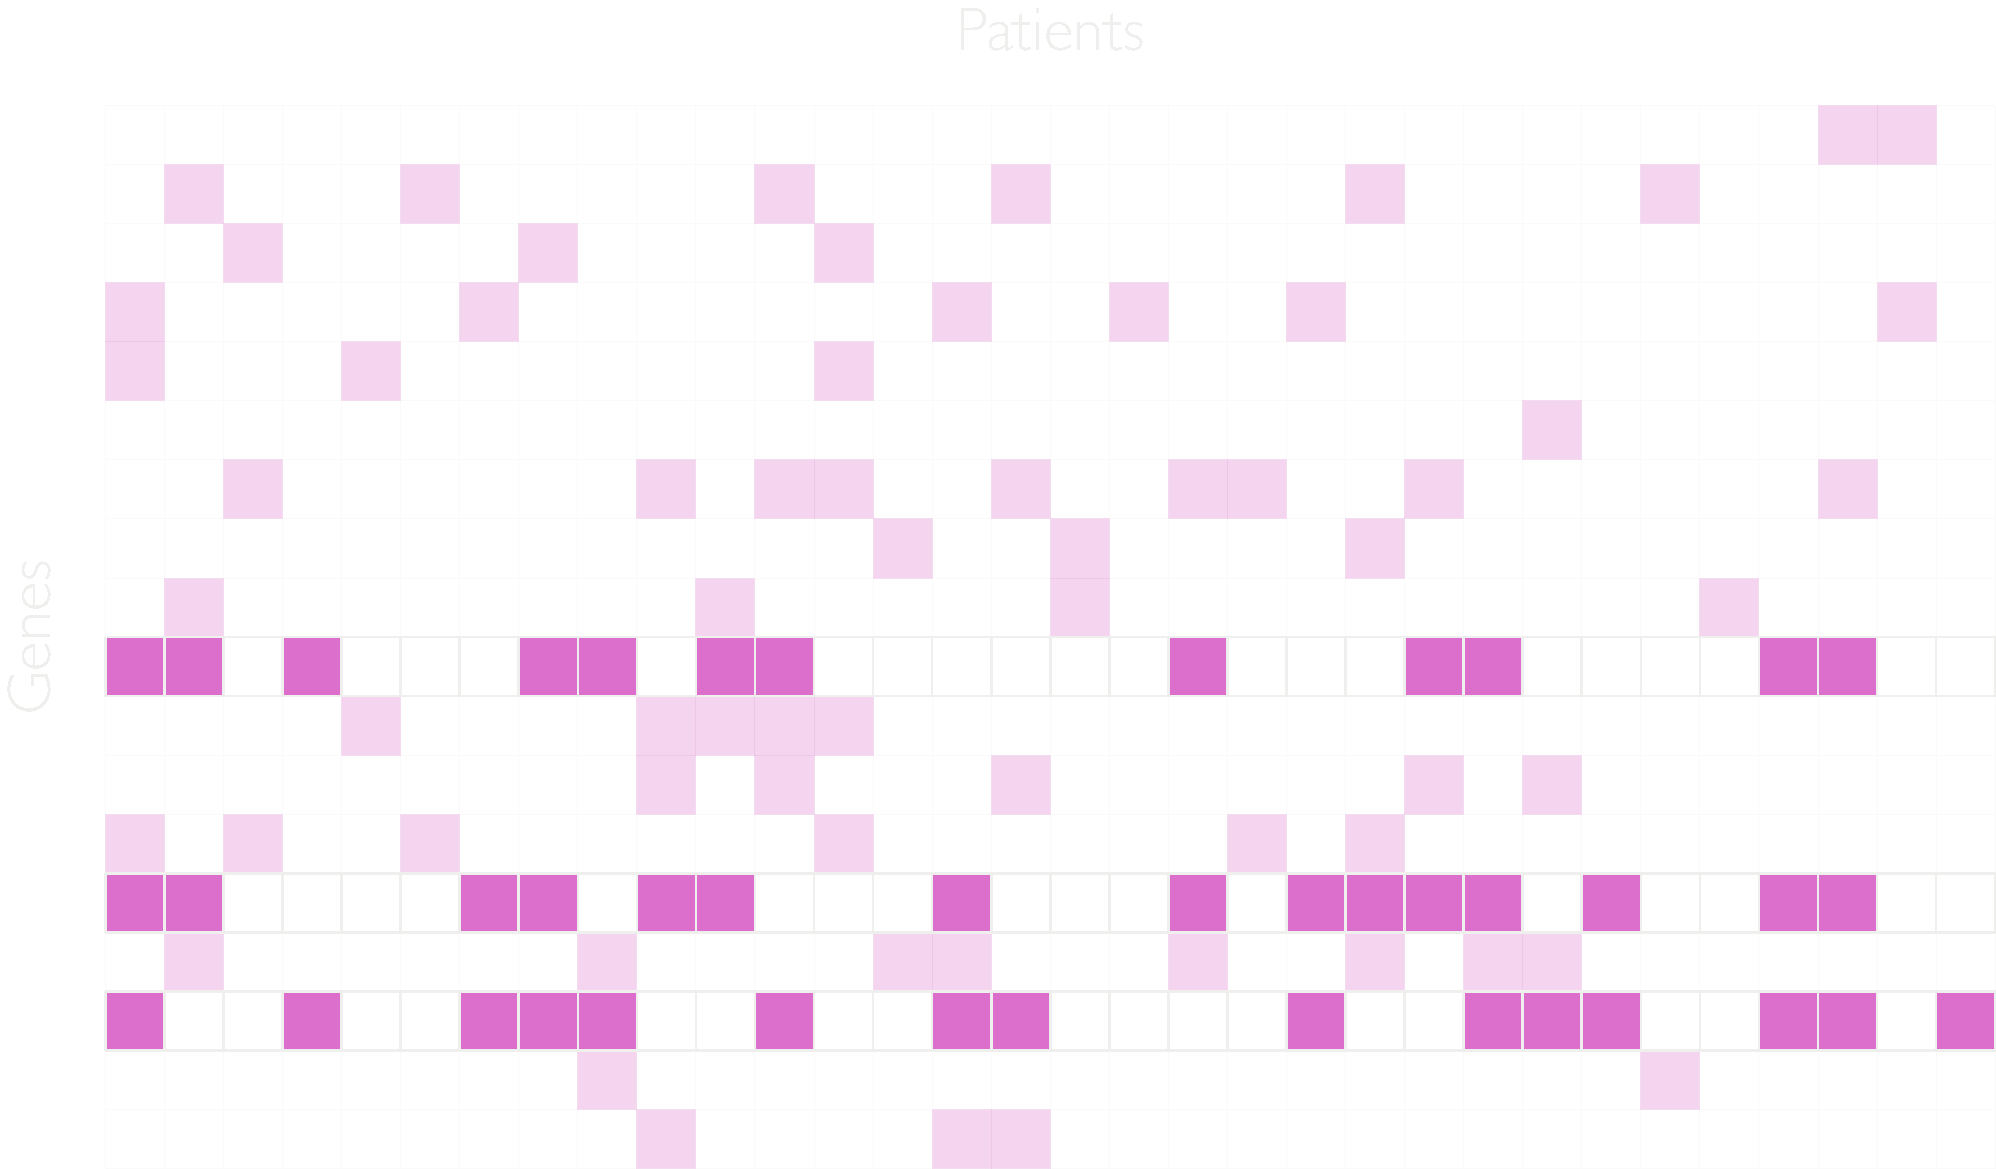
\includegraphics[width=\textwidth]{figures/grid_genes_cooc.pdf}
\end{frame}

\begin{frame}{Modeling teams}
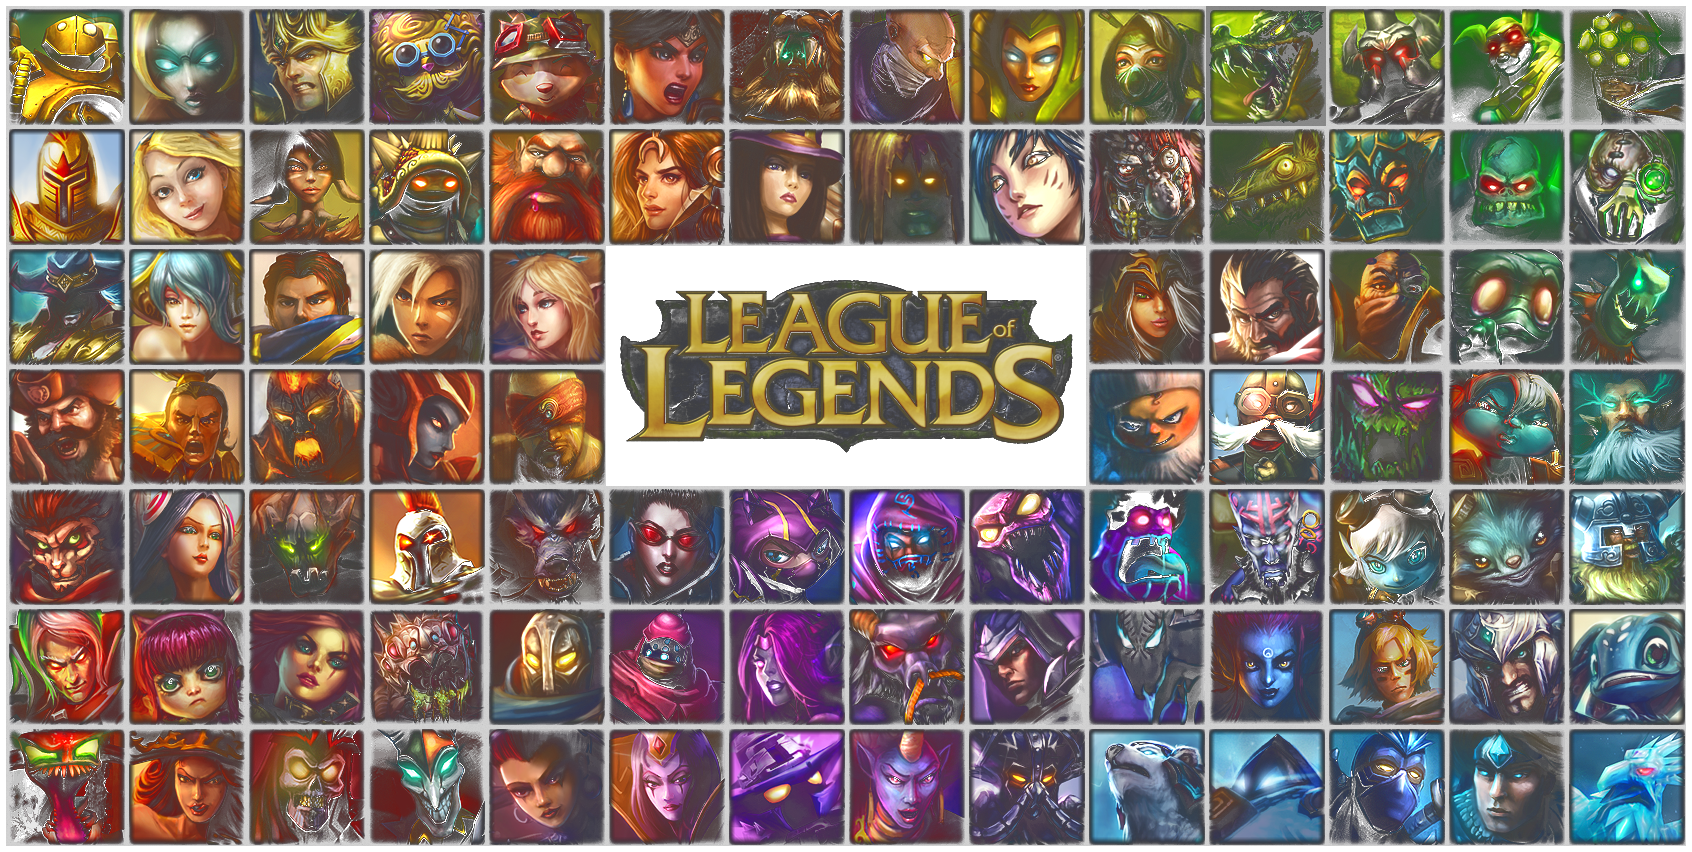
\includegraphics[width=\textwidth]{figures/champions_transparent.png}\\
\qsource{\texttt{euw.leagueoflegends.com}}
\end{frame}

\begin{frame}{Modeling teams}
\centering
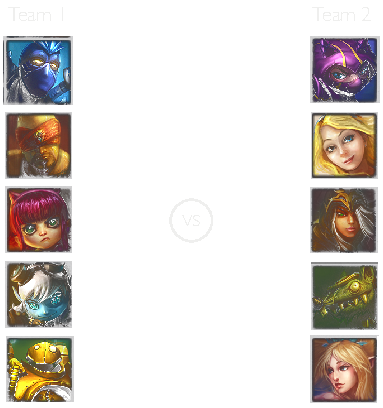
\includegraphics[height=3in]{figures/champions5v5.pdf}
\end{frame}

\begin{frame}{Modeling teams}
\centering
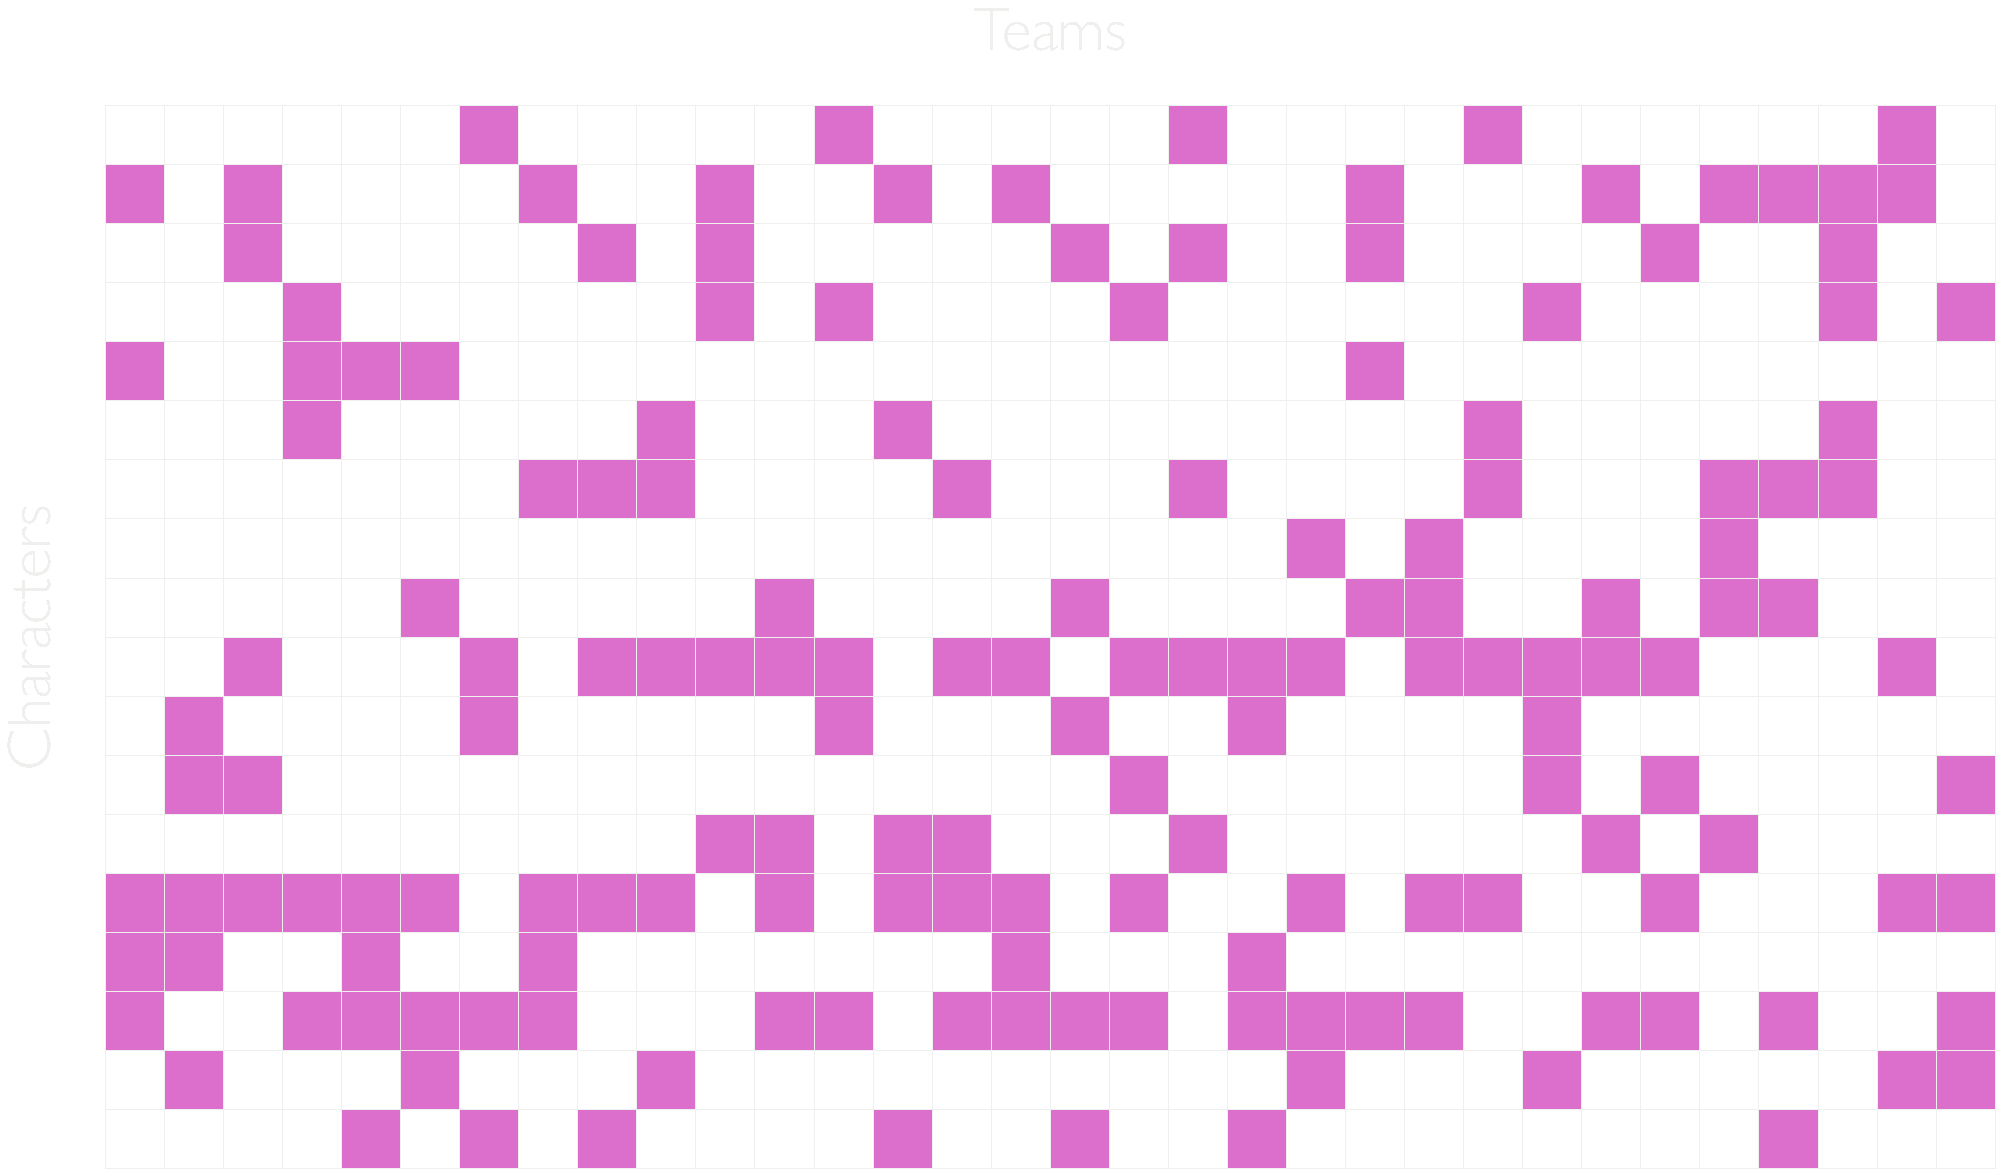
\includegraphics[width=\textwidth]{figures/grid_hots.pdf}
\end{frame}

\begin{frame}{When Gibbs fails}
\centering
\only<1>{
\includegraphics[width=4in]{figures/bottleneck0.pdf}}%
\only<2>{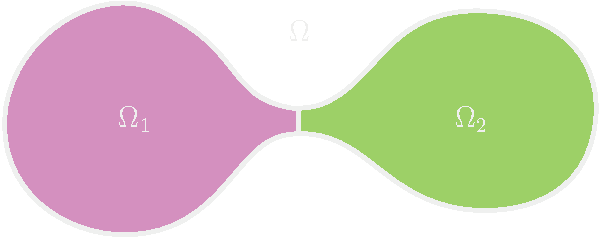
\includegraphics[width=4in]{figures/bottleneck1.pdf}}%
\only<3>{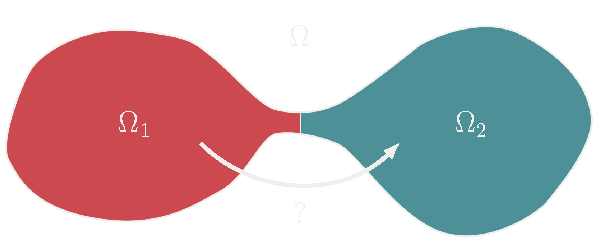
\includegraphics[width=4in]{figures/bottleneck2.pdf}}
\end{frame}

\end{document}
